\documentclass[a4paper]{article}
\usepackage{amsmath, amssymb, bm}
\usepackage[margin=1in]{geometry}
\usepackage{graphicx}

\DeclareMathOperator*{\argmax}{arg\,max}

\begin{document}
	\begin{titlepage}
		\centering
		{\huge \bf Assignment 4\par}
		\vspace{1cm}
		{\Large Computational Intelligence, SS2018\par}
		\vspace{1cm}
		\begin{tabular}{|l|l|l|}
			\hline
			\multicolumn{3}{|c|}{\textbf{Team Members}}   \\ \hline
			Last name & First name & Matriculation Number \\ \hline
			Lee       & Eunseo     & 11739623             \\ \hline
			Shadley   & Alex       & 11739595             \\ \hline
			Lee       & Dayeong    & 11730321             \\ \hline
		\end{tabular}
	\end{titlepage}

\section{Maximum Likelihood Estimation of Model Parameters}
\subsection{Find out which is the anchor with exponentially distributed measurements}

To find out which anchor is with exponentially distributed measurements, I used Kolmogorov-Smirnov test.\newline
The following picture is the KS test statistic with parameter "expon", which is exponential distribution, for each anchor.

\begin{figure}[h]
	\begin{center}
	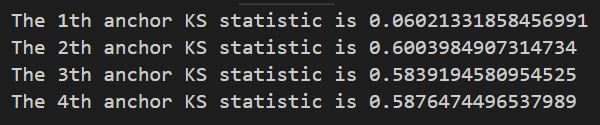
\includegraphics[width=0.5\textwidth]{kstest.jpg}
	\caption{KS test statistic}
	\end{center}
\end{figure}

If KS statistic is close to 0, it means that the dataset is similar with the parameter distribution. \textbf{First anchor} KS statistic is close to 0. Therefore, first anchor follows exponential distribution because above KS test parameter is exponential distribution.

\subsection{Analytically derive the maximum likelihood solution for the exponential distribution}

\newcommand{\prip}{p(r_i|p)}
\newcommand{\ridi}{r_i-d_i(p)}
\newcommand{\signa}{\sum\limits_{i=1}^{N_A}}
\newcommand{\mulna}{\prod\limits_{i = 1}^{N_A}}

To find the parameter $\lambda$ which maximizes the likelihood, we should differentiate the maximum likelihood function and set the Differential equation as 0. Then, we can find thethe parameter $\lambda$ in terms of position data($\ridi$).\\
\noindent
First, the maximum likelihood function is like this.\\
\begin{equation}
\hat{p}_{ML} = \arg\max\limits_{p}p(r|p) = \arg\max\limits_{p}\mulna\prip\\
\end{equation}

\noindent
To find the maximum likelihood, we should differentitiate the maximum likelihood.\\
\begin{equation}
\mulna\prip =\mulna\lambda\exp^{-\lambda(\ridi)} = (\lambda)^{NA}\exp^{-\lambda\signa(\ridi)}
\end{equation}

\noindent
To make the calculation easy, take the natural log on both side.
\begin{equation}
\ln\mulna\prip = N_A \ln\lambda - \lambda\signa(\ridi)
\end{equation}

\noindent
To find the $\lambda$, which maximizes the likelihood function, we should differntiate the function in terms of $\lambda$ and set the equation as a. 
\begin{equation}
\frac{\partial(\ln\mulna\prip)}{\partial \lambda} = \frac{N_A}{\lambda} - \signa(\ridi) =0
\end{equation}

\noindent
Finally, we get the parameter $\lambda$ (solution).
\begin{equation}
\lambda = \frac{N_A}{\signa(\ridi)} = \frac{1}{\overline{\ridi}} = \frac{1}{\mu}
\end{equation}
\clearpage

\subsection{Estimate the parameters of the measurement models}
\subsubsection{Scenario 1: Measurements of all anchors follow the Gaussian model.}
\begin{figure}[h]
	\begin{center}
		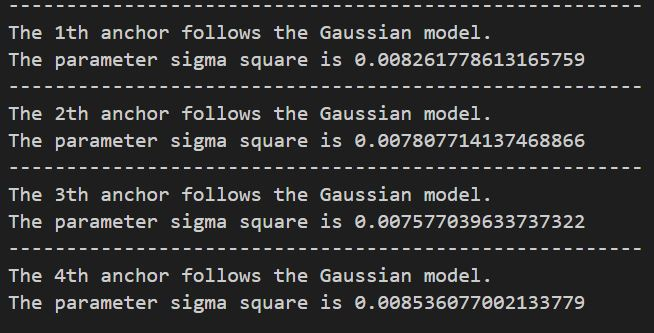
\includegraphics[width=0.5\textwidth]{scenario1param.jpg}
		\caption{Parameters for each anchor}
	\end{center}
\end{figure}
\subsubsection{Scenario 2: Measurements of one anchor follow the Exponential model, the other ones follow the Gaussian model.}
\begin{figure}[h]
	\begin{center}
		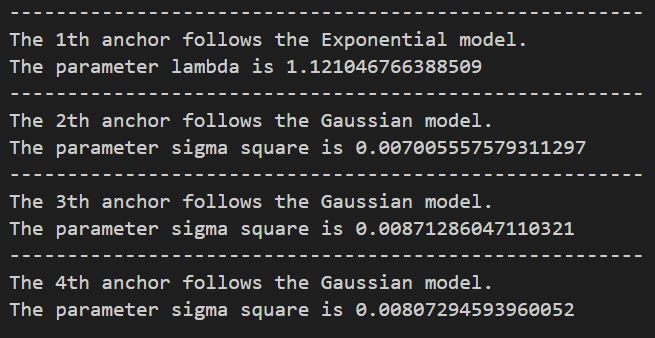
\includegraphics[width=0.5\textwidth]{scenario2param.jpg}
		\caption{Parameters for each anchor}
	\end{center}
\end{figure}

\subsubsection{Scenario 3: Measurements of all anchors follow the Exponential model.}
\begin{figure}[h]
	\begin{center}
		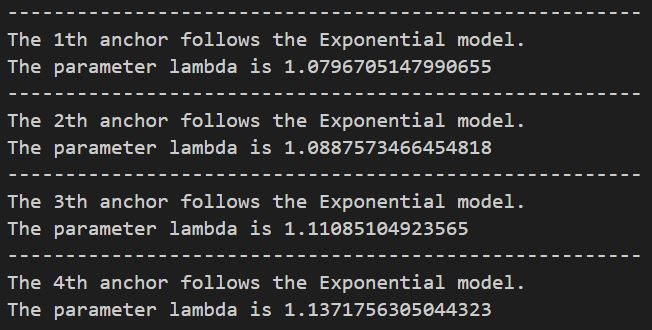
\includegraphics[width=0.5\textwidth]{scenario3param.jpg}
		\caption{Parameters for each anchor}
	\end{center}
\end{figure}

\section{Estimation of the Position}
\subsection{Least-Squares Estimation of the Position}
\subsubsection{Show analytically that the least-squares estimator of the position is equivalent to the maximum likelihood estimator for Gaussian distribution model}

\noindent
The maximum likelihood estimatior for guassian distribution model is like this.
\newcommand{\maxp}{\arg\max\limits_{p}}
\newcommand{\minp}{\arg\min\limits_{p}}
\begin{equation}
\hat{p}_{ML} = \arg\max\limits_{p}p(r|p) = \maxp\mulna\prip =\maxp (\frac{1}{\sqrt{2\pi\sigma^2}})^{N_A}\exp^{-\frac{1}{2\sigma^2}\signa(\ridi)^2} \\
\end{equation}

\noindent
Maximizing the function (6) is the same as minizing the negative of its logarithm. Therfore, the equation(6) is equivalent to the equation (7).
\begin{equation}
\minp(-\ln((\frac{1}{\sqrt{2\pi\sigma^2}})^{N_A}\exp^{-\frac{1}{2\sigma^2}\signa(\ridi)^2})) = \minp(N_A\ln\sqrt{2\pi\sigma^2}+\frac{1}{2\sigma^2}\signa(\ridi)^2)
\end{equation}
Since $N_A$ and $\sigma$ are constant, the equation(7) can be simplified to equation (8).
\begin{equation}
\minp\signa(\ridi)^2 = \minp ||r-d(p)||^2
\end{equation}
Then, the equation(8) is the least square estimator of the position.\\ That is, we proved that the least square estimator of the position is equivalent to the maximum likelihood estimator for Gaussian distribution model.

\subsubsection{Implement the Gauss-Newton algorithm}

First, we just set the tolerance as 0.000005 and the max\_iteration as 10.\\
Then, we iterate with new start point(selected within the anchors square with uniform distribution) through the measurements.
\begin{figure}[h]
	\begin{center}
		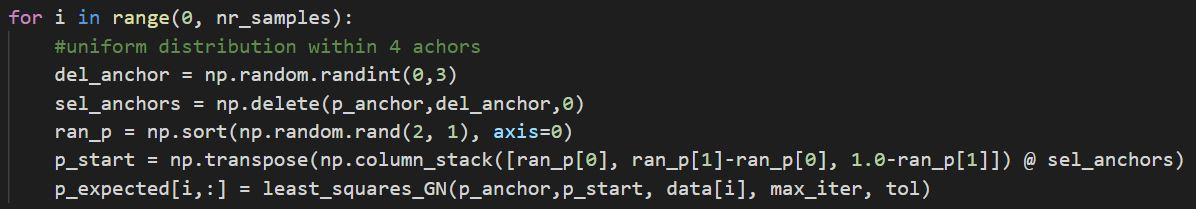
\includegraphics[width=0.5\textwidth]{gauss_newton.jpg}
		\caption{Main loop for iterating measurements}
	\end{center}
\end{figure}\\
The following figure is the main code of Gauss\_Newton.\\
\begin{figure}[h]
	\begin{center}
		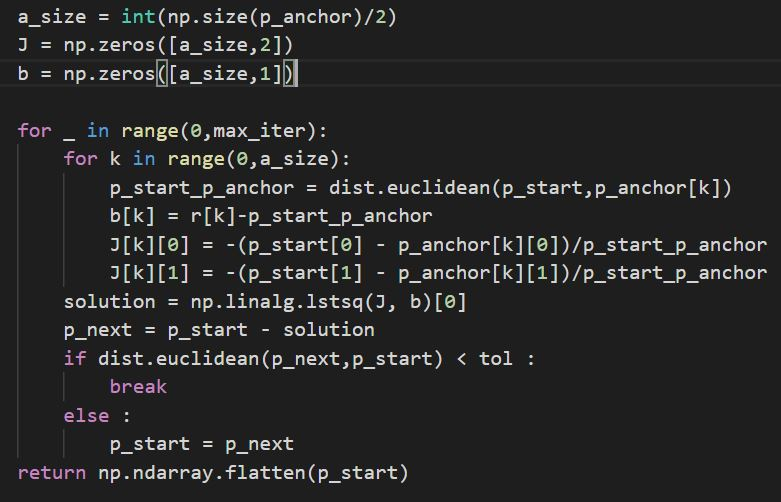
\includegraphics[width=0.4\textwidth]{least_square.jpg}
		\caption{Least\_square with Gauss\_Newton}
	\end{center}
\end{figure}

J is jacobian matrix and b is $(r-d(\hat{p}\textsuperscript{(t)}))$.
Using 'np.linalg.lstsq', which is the least square solver, we get the solution. Then, we update the position of agent and check tolerence and max iteration.

\clearpage
\subsubsection{Evaluate your estimation algorithm : Scenario 1}
\begin{figure}[h]
	\begin{center}
		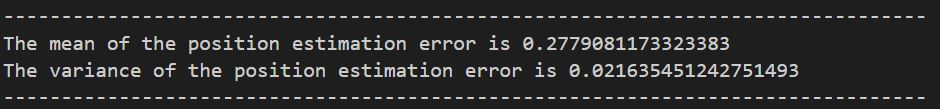
\includegraphics[width=0.5\textwidth]{mean_variance_error1.jpg}
		\caption{The mean and variance of the position estimation error}
	\end{center}
\end{figure}
\begin{figure}[h]
	\begin{center}
		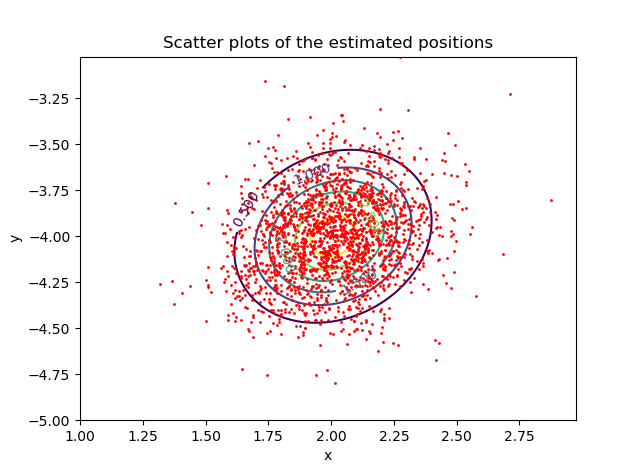
\includegraphics[width=0.5\textwidth]{plotcon1.png}
		\caption{Scatter plots of the estimated positions with contourlines}
	\end{center}
\end{figure}
The estimated positions looks like following Gaussian distribution.
\begin{figure}[h]
	\begin{center}		
		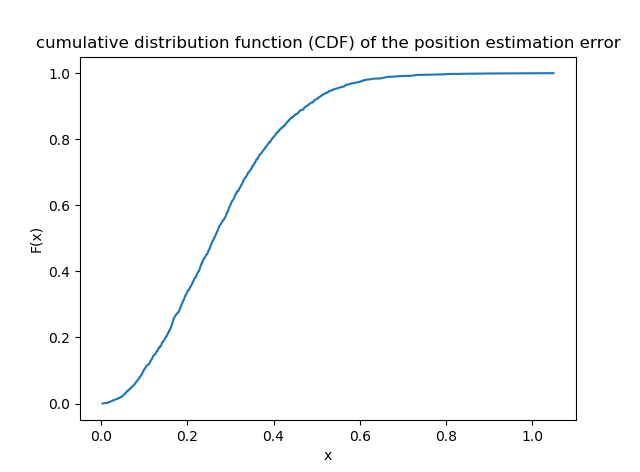
\includegraphics[width=0.5\textwidth]{CDF1.png}
		\caption{cumulative distribution function (CDF) of the position estimation error}
	\end{center}
\end{figure}

The probability that the position estimation error is smaller than 0.4, is 0.8.

\clearpage
\subsubsection{Evaluate your estimation algorithm : Scenario 2}
\begin{figure}[h]
	\begin{center}
		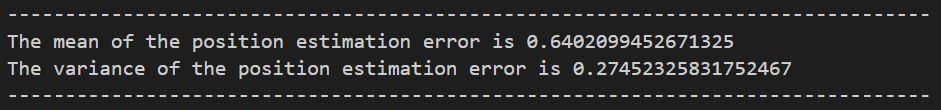
\includegraphics[width=0.5\textwidth]{mean_variance_error2.jpg}
		\caption{The mean and variance of the position estimation error}
	\end{center}
\end{figure}
\begin{figure}[h]
	\begin{center}
		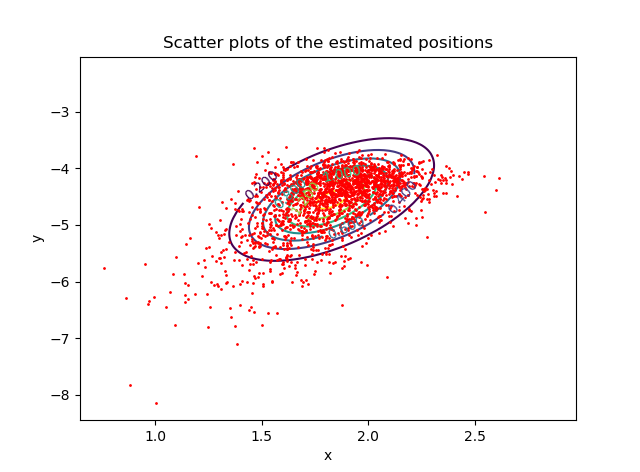
\includegraphics[width=0.5\textwidth]{plotcon2.png}
		\caption{Scatter plots of the estimated positions with contourlines}
	\end{center}
\end{figure}
The estimated positions doesn't look like following Gaussian distribution because the graph is skewed to the direction bottom left.
\begin{figure}[h]
	\begin{center}		
		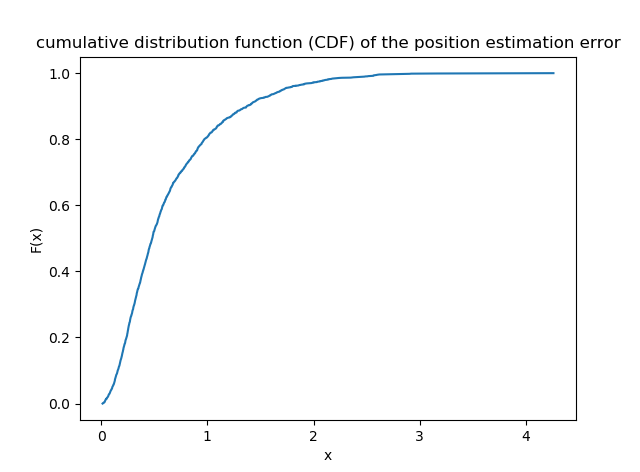
\includegraphics[width=0.5\textwidth]{CDF2.png}
		\caption{cumulative distribution function (CDF) of the position estimation error}
	\end{center}
\end{figure}

The probability that the position estimation error is smaller than 0.4, is 0.35.




\clearpage
\subsubsection{Evaluate your estimation algorithm : Scenario 3}
\begin{figure}[h]
	\begin{center}
		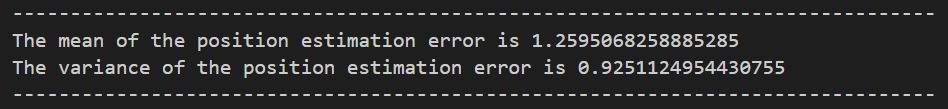
\includegraphics[width=0.5\textwidth]{mean_variance_error3.jpg}
		\caption{The mean and variance of the position estimation error}
	\end{center}
\end{figure}
\begin{figure}[h]
	\begin{center}
		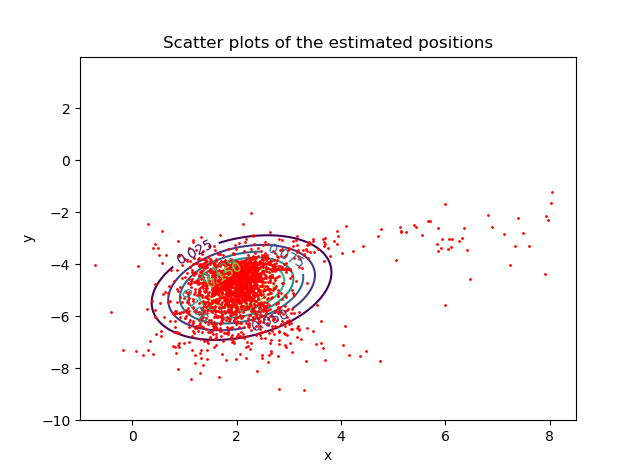
\includegraphics[width=0.5\textwidth]{plotcon3.png}
		\caption{Scatter plots of the estimated positions with contourlines}
	\end{center}
\end{figure}
The estimated positions doens't look like following Gaussian distribution becuase lots of esimated positions are scattered outside of contoured region.
\begin{figure}[h]
	\begin{center}		
		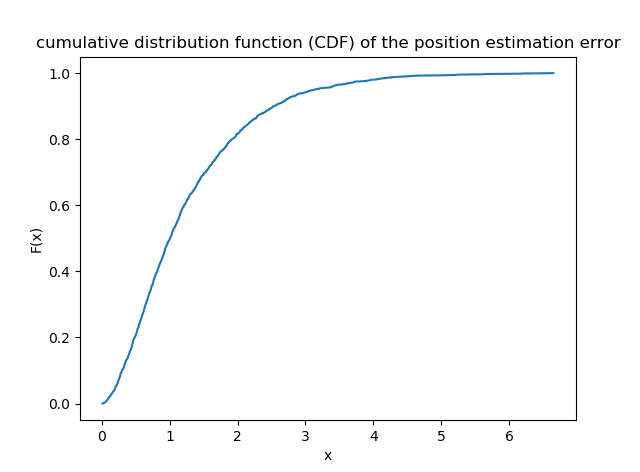
\includegraphics[width=0.5\textwidth]{CDF3.png}
		\caption{cumulative distribution function (CDF) of the position estimation error}
	\end{center}
\end{figure}

The probability that the position estimation error is smaller than 0.4, is 0.1.\\

$\bullet$ \textbf{Comparision of the probability that the position estimation error is smaller than 0.4}\\

\hspace{0.5cm} Scenario 1(0.8) $>$ Scenario 2(0.35) $>$ Scenario 3(0.1)\\

\hspace{0.5cm} The probability of scenario 1 is the smallest. The reason is that measurements of 4 anchors follow the Gaussian model. The least square esimation works well on gaussian model so the performance of scenario 1 is the highest. In the case of scenario 2, there exists one exponential model so the performance is lower than scenario 1 because an exponential model doesn't work well on least square estimation. In the case of scenario 3, it consists of 4 exponential models so it ranks the lowest among 3 scenarios.

\clearpage
\subsubsection{Consider scenario 2.: Try neglecting the anchor with the exponentially distributed measurements at all}
\begin{figure}[h]
	\begin{center}
		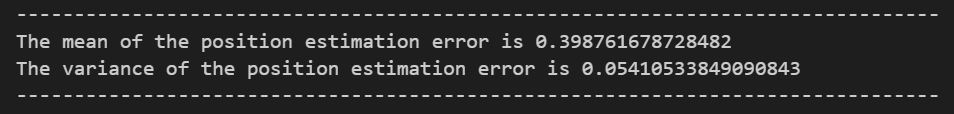
\includegraphics[width=0.5\textwidth]{mean_variance_neglect.jpg}
		\caption{The mean and variance of the position estimation error}
	\end{center}
\end{figure}
\noindent
The mean value is decreased from 0.64 to 0.39.\\
The varaiance value is decreased from 0.27 to 0.05.\\
\begin{figure}[h]
	\begin{center}
		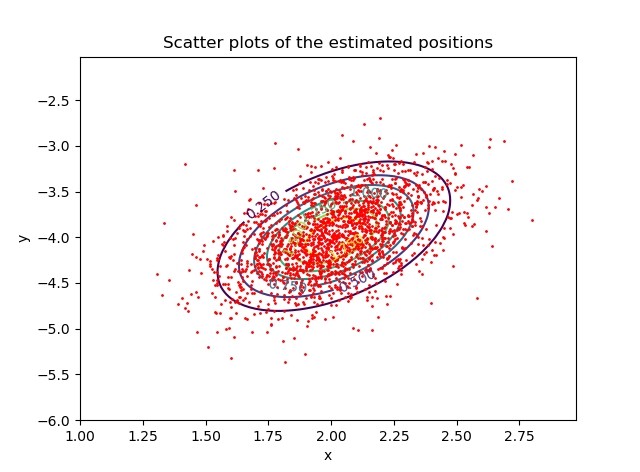
\includegraphics[width=0.5\textwidth]{neglect1.png}
		\caption{Scatter plots of the estimated positions with contourlines}
	\end{center}
\end{figure}

\noindent
The estimated positions looks like following Gaussian distribution.
\begin{figure}[h]
	\begin{center}		
		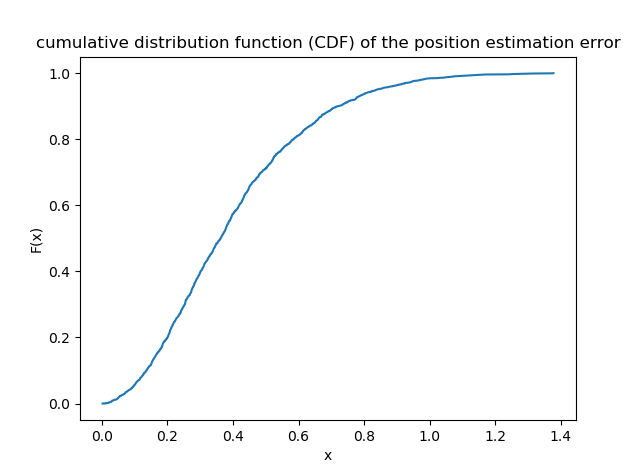
\includegraphics[width=0.5\textwidth]{neglect2.png}
		\caption{cumulative distribution function (CDF) of the position estimation error}
	\end{center}
\end{figure}

The probability that the position estimation error is increased from 0.35 to 0.7.\\
After neglecting the anchor with exponential distribution, the mean, variance are decreased, the scatter plot looks like gaussian distribution and the probability, which the error is smaller than 0.4, is decrased. That is, the performance of the algorithm is improved.
\clearpage

\subsection{Numerical Maximum-Likelihood Estimation of the Position}

\subsubsection*{Part 1}
An alternative to iterative Maximum Likelihood estimation is a Numerical approach.  With this approach, our joint likelihood function $p(\bm{r}|\bm{p})$ is evaluated at every point of a fine grid, 5 cm resolution in this case, and the highest value taken as the Maximum Likelihood.  We use this method with scenario 3, where the measurements from all anchors follow an exponential distribution, so we use the following distribution function

\[
	p(\bm{r_i}|\bm{p}) = 
	\begin{cases}
		\lambda _i e^{-\lambda _i (r_i - d_i(\bm{p}))} & r_i \geq d_i(\bm{p}) \\
		0 & \text{else} \\
	\end{cases}
\]

\[
p(\bm{r}|\bm{p}) = \prod_{i=1}^N p(\bm{r_i}|\bm{p}) ,
\]

where $N$ is the number of anchors, and $d_i(\bm{p})$ is the euclidean distance between point $\bm{p}$ and anchor $i$.  One can see that the joint likelihood $p(\bm{r}|\bm{p})$ is obtained by taking the product of the individual likelihoods of each anchor.

\begin{figure}[h]
	\begin{center}
		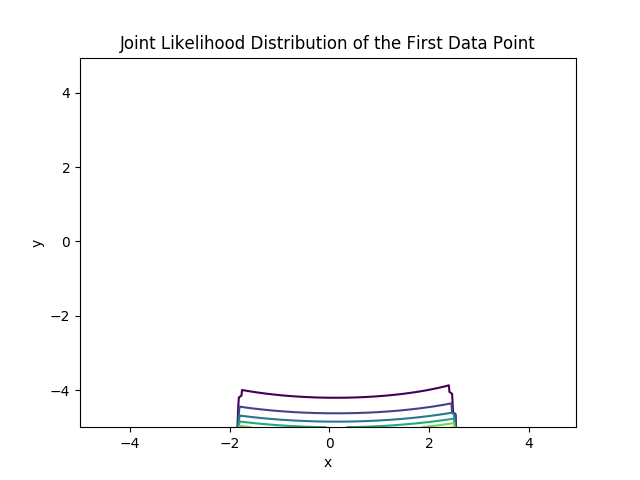
\includegraphics[width=0.5\textwidth]{joint_likelihood_dist.png}
		\caption{Joint likelihood of the first data point}
	\end{center}
\end{figure}

The maximum found here is not the true location of $\bm{p}$.  While it is possible, since $\bm{p}$ lies along the compute grid, the noisiness of the data makes finding the actual point very unlikely.  Nonetheless, the maximum 

The numerical approach is better suited than gradient ascent to the exponential distribution.  One key issue with gradient ascent is that it requires a non-zero gradient to be effective.  Since the exponential distribution is described as 0 where $r_i < d_i(\bm{p})$, large areas of the solution space have a gradient of 0.  If the gradient ascent algorithm were to start in one such region, it would become stuck and unable to converge.  The peicewise definition of the exponential distribution also means that it is not differentiable at all points, posing further difficulties.

\subsubsection*{Part 2}

The method in the previous section is then applied to each available measurement.  The likelihood for each measurement is computed over a grid, and the maximum value over this grid taken as the estimated Maximum Likelihood.

\begin{figure}[h]
	\begin{center}
		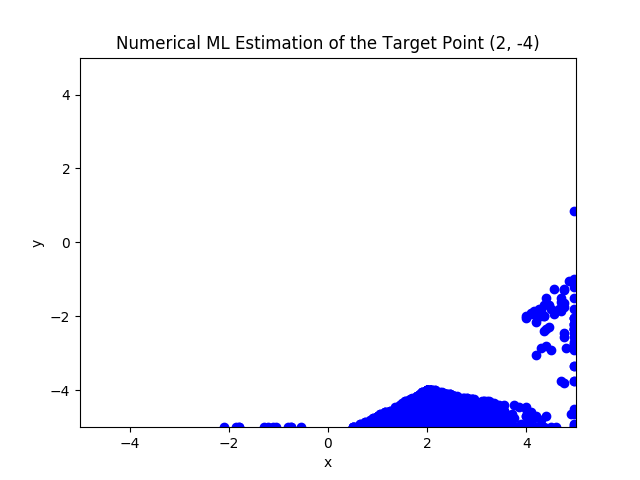
\includegraphics[width=0.5\textwidth]{numerical_mle.png}
		\caption{Numerical MLE for Scenario 3}
	\end{center}
\end{figure}

The numerical method does have drawbacks.  Compared to iterative models, it is very computationally intensive, resulting in much slower solutions.  This is because a numerical estimation must perform a computation on every point on a grid covering the solution space.  Searching a particularly large solution space quickly becomes too computationally expensive to have any real-world application.  The resolution of the computation grid can be decreased to reduce the required number of computations, but this in turn will produce less accurate results.

Nonetheless, this is a fair comparison since both approaches produce a Maximum Likelihood estimates, albeit with strikingly dissimilar methods.  In this sense the numerical approach is a true Maximum Likelihood Estimator.

To improve accuracy, it may be tempting to consider not just one measurement, but all available measurements.  Theoretically, one could take the product of all joint distributions, one for each measurement, to produce a much more accurate estimate.  A potential issue with this is that joint distributions typically hold small values; taking the product of 2000 such functions may produce numbers too small to be efficiently handled by computers.  Additionally, in real-world applications it is unlikely that a large volume of relevant measurements would be available at a given instant.

\subsubsection*{Part 3}

Another method, referred to here as the 'Bayesian Method' involves including prior knowledge about the point being estimated to increase accuracy.  It follows the formula

\[
\hat{p}_Bayes = \argmax _p p(\bm{r}|\bm{p}) p(\bm{p}) , 
\]

where $p(\bm{p})$ is a Gaussian distribution centered on $\bm{p}$ with covariance matrix $\sigma$ = diag{$\sigma ^2$} and $\sigma = 1$.

\begin{figure}[h]
	\begin{center}
		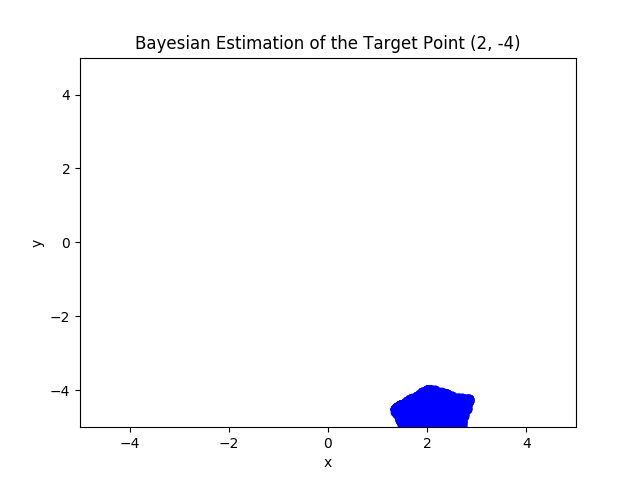
\includegraphics[width=0.5\textwidth]{bayesian_mle.png}
		\caption{Bayesian MLE for Scenario 3}
	\end{center}
\end{figure}

It should be noted that while this approach looks promising, it relies on the prior knowledge of the point we are trying to estimate.

\end{document}